%============================================================================%
% Antoine Gé́ré (gereantoine@gmail.com). 
%============================================================================%                                                     

%-- CLASS ------------------------------------------------------------------%

\documentclass[9pt]{beamer} 

\pdfoutput=1 

\makeatletter 

%-- PACKAGES ----------------------------------------------------------------%

\usepackage{amscd}
\usepackage{amsmath}
\usepackage{amsthm}
\usepackage{amsxtra}
\usepackage{array} 

\usepackage[english]{babel} 

\usepackage{cancel}
\usepackage{color}

\usepackage{enumitem}

\usepackage{fancyhdr}
\usepackage[T1]{fontenc} 

\usepackage{geometry} 
\usepackage{graphicx} 

\usepackage{hyperref} 

\usepackage[utf8]{inputenc} 

\usepackage{letltxmacro}
\usepackage{lmodern}

\usepackage{manfnt}
\usepackage{multicol} 

\usepackage[numbers,sort]{natbib}

\usepackage{pgf}

\usepackage{setspace} 

\usepackage{tikz}

\usepackage{url}
 
\usepackage{wasysym}
\usepackage{wrapfig}

\usepackage{xcolor}

%-- THEME -------------------------------------------------------------------%

\mode<presentation>
{

  %== NAVIGATION SYMBOLS ======================================================%    

  \setbeamertemplate{navigation symbols}{}
  
  %== TITLE PAGE ==============================================================%    

  %\newcommand\subtitle[1]{\def\insertsubtitle{#1}}
  %\subtitle{}

  \newcommand\coauthor[1]{\def\insertcoauthor{#1}}
  \coauthor{}

  \newcommand\conference[1]{\def\insertconference{#1}}
  \conference{}

  \newcommand\shortconference[1]{\def\insertshortconference{#1}}
  \shortconference{}

  \newcommand\paper[1]{\def\insertpaper{#1}}
  \paper{}

  \newcommand\LogoUniv[1]{\def\insertLogoUniv{#1}}
  \paper{}
  
  \newcommand\TitlePic[1]{\def\insertTitlePic{#1}}
  \paper{}

  \pgfdeclareverticalshading[title page.bg]{beamer@titleshade}{\paperwidth}{%
    color(0pt)=(black!30!white);
    color(3pt)=(black!60!white);
    color(3pt)=(title page.bg);
    color(126pt)=(title page.bg);
    color(126pt)=(black!60!white);
    color(129pt)=(black!30!white)}
  
  \defbeamertemplate*{title page}{gottingen14}[1][]
  {%
    \hbox{%
      %
      \leavevmode%
      \advance\beamer@leftmargin by -12bp%
      \advance\beamer@rightmargin by -12bp%
      \beamer@tempdim=\textwidth%
      \advance\beamer@tempdim by \beamer@leftmargin%
      \advance\beamer@tempdim by \beamer@rightmargin%
      \hskip-\Gm@lmargin%
      %
      \hbox{%
	\setbox%
	\beamer@tempbox=\hbox{%
	%
	\begin{minipage}[b]{\paperwidth}%
	  \vbox{}%
	  \leavevmode%
	  \center{%
	    {\usebeamerfont{title}\inserttitle} \\[3pt]
	    {\usebeamerfont{author}\color{black}\insertauthor}\\[1pt]%
	    {\usebeamerfont{institute}\color{black}\insertinstitute}\\[-2pt]%
	    {\usebeamerfont{institute}\color{black}\insertdate}\\[-2pt]%
	  }%
	  \strut%
	  \par%
	  \vbox{}%
	\end{minipage}%
	}%
	%
	\beamer@tempdim=\ht\beamer@tempbox%
	\advance\beamer@tempdim by 115pt%
	%
	\begin{pgfpicture}{0pt}{0pt}{\paperwidth}{\beamer@tempdim}
	  \pgfsetfillopacity{0.8}
	  \pgftext[left,base]{\pgfuseshading{beamer@titleshade}}
	\end{pgfpicture}
	%
	\hskip-\paperwidth%
	\box\beamer@tempbox%
      }%
    }%
  }

  %== TEMPLATE ================================================================% 
 
  \setbeamertemplate{title page}[gottingen14][colsep=-4bp,rounded=false]
  \setbeamertemplate{sections/subsections in toc}[ball]
  \setbeamertemplate{items}[ball]
  \setbeamertemplate{blocks}[default]
  \setbeamertemplate{part page}[default][colsep=-4bp,rounded=false]
    
  %== COLOR ===================================================================% 
  
  \setbeamercolor{title page}{bg=white!96!black,fg=red!62!black}
  \setbeamercolor{frametitle}{bg=white,fg=red!60!black}
  \setbeamercolor{subsection in head/foot}{bg=white!95!black,fg=red!60!black}
  \setbeamercolor{author in head/foot}{bg=white,fg=red!60!black}
  \setbeamercolor{title in head/foot}{bg=white,fg=red!60!black}
  \setbeamercolor{normal text}{black}
  \setbeamercolor{headline@color}{bg=black,fg=green}
  \setbeamercolor{block title}{bg=black!20!white,fg=red!60!black}
  \setbeamercolor{block body}{bg=black!20!white,fg=black}
  \setbeamercolor{block body alerted}{bg=black!40!white,fg=black}
  \setbeamercolor{block title alerted}{bg=black!40!white,fg=black}
  \setbeamercolor{block body example}{bg=black!10!white,fg=black}
  \setbeamercolor{block title example}{bg=black!10!white,fg=red!60!black}
  \setbeamercolor{button}{bg=black!50!white,fg=white}
  \setbeamercolor{sidebar}{bg=black,fg=white}
  \setbeamercolor{palette sidebar primary}{bg=black,fg=white}
  \setbeamercolor{palette sidebar secondary}{bg=black,fg=white}
  \setbeamercolor{palette sidebar tertiary}{bg=black,fg=white}
  \setbeamercolor{palette sidebar quaternary}{bg=black,fg=white}
  \setbeamercolor{titlelike}{bg=green,fg=white}
  \setbeamercolor{separation line}{white}
  \setbeamercolor{fine separation line}{white}

  %== FONT ====================================================================% 
  
  \setbeamerfont{frametitle}{size={\normalsize},series={\bf}}
  \setbeamerfont{block title}{size={},series={}}
  \setbeamerfont{block body}{size={},series={}}
  \setbeamerfont{block title example}{size={},series={}}
  \setbeamerfont{block body example}{size={},series={}}
  \setbeamerfont{title}{size={\LARGE},series={\bf}}
  \setbeamerfont{subtitle}{size={\large},series={\bf}}
  \setbeamerfont{author}{size={\Large},series={\bf}}
  \setbeamerfont{institute}{size={\normalsize},series={}}
  \setbeamerfont{conference}{size={\large},series={}}
  \setbeamerfont{date}{size={\normalsize},series={}}
  \setbeamerfont{coauthor}{size={\normalsize},series={\bf}}
  \setbeamerfont{paper}{size={\normalsize},series={\tt}}

  %== COVERED =================================================================% 
  
  \setbeamercovered{transparent}
    
  %== SHADOWS =================================================================% 

  \AtBeginDocument{%
    \pgfdeclareverticalshading{beamer@topshade}{\paperwidth}{%
      color(0pt)=(bg);%
      color(4pt)=(black!50!bg)}%
    \pgfdeclareverticalshading{beamer@bottomshade}{\paperwidth}{%
      color(0pt)=(black!50!bg);%
      color(4pt)=(bg)}%
    \pgfdeclarehorizontalshading{beamer@rightshade}{\paperwidth}{%
      color(0pt)=(black!50!bg);%
      color(4pt)=(bg)}%
    \pgfdeclarehorizontalshading{beamer@leftshade}{\paperwidth}{%
      color(0pt)=(black!50!bg);%
      color(4pt)=(bg)}%
  }%

  %== FRAME TITLE =============================================================% 

    \pgfdeclareverticalshading[frametitle.bg]{beamer@frametitleshade}{\paperwidth}
    {%
      color(0pt)=(frametitle.bg);
      color(36pt)=(frametitle.bg)
    }%

    \defbeamertemplate*{frametitle}{nosplit theme}
    {%
      \nointerlineskip%
      \vskip-2.5pt%
      \hbox{\leavevmode
        \advance\beamer@leftmargin by -12bp%
        \advance\beamer@rightmargin by -12bp%
        \beamer@tempdim=\textwidth%
        \advance\beamer@tempdim by \beamer@leftmargin%
        \advance\beamer@tempdim by \beamer@rightmargin%
        \hskip-\Gm@lmargin\hbox{%
          \setbox\beamer@tempbox=\hbox{
          \begin{minipage}[b]{\paperwidth}%
              \vbox{}%
              \vskip0ex%
              \leftskip0.3cm%
              \rightskip0.3cm plus1fil\leavevmode
              \insertframetitle%
              \ifx\insertframesubtitle\@empty%
                \strut\par%
              \else
                \par{\usebeamerfont*{framesubtitle}{\insertframesubtitle}\strut\par}%
              \fi%
              \vskip5pt%
              \nointerlineskip
              \vbox{}%
              \end{minipage}}%
          \beamer@tempdim=\ht\beamer@tempbox%
          \advance\beamer@tempdim by 2pt%
          \begin{pgfpicture}{0pt}{0pt}{\paperwidth}{\beamer@tempdim}
            \usebeamercolor{frametitle}
            \pgfpathrectangle{\pgfpointorigin}{\pgfpoint{\paperwidth}{\beamer@tempdim}}
            \pgfusepath{clip}
            \pgftext[left,base]{\pgfuseshading{beamer@frametitleshade}}
          \end{pgfpicture}
          \hskip-\paperwidth%
          \box\beamer@tempbox%
        }%
        \hskip-\Gm@rmargin%
      }%
      \nointerlineskip
        \vskip-0.2pt
        \hbox to\textwidth{\hskip-\Gm@lmargin\pgfuseshading{beamer@topshade}\hskip-\Gm@rmargin}
        \vskip-2pt
    }

  %== FOOTLINE ================================================================%    

  \newcommand{\backupbegin}{
    \newcounter{framenumberappendix}
    \setcounter{framenumberappendix}{\value{framenumber}}
  }

  \newcommand{\backupend}{
    \addtocounter{framenumberappendix}{-\value{framenumber}}
    \addtocounter{framenumber}{\value{framenumberappendix}} 
  }

  \defbeamertemplate*{footline}{nosplit theme}{%
    \vskip1pt
    \pgfuseshading{beamer@bottomshade}
    \vskip1.5pt
    \leavevmode%
    \hbox{%
      \begin{beamercolorbox}[wd=.2\paperwidth,center]{footline@color}%
	\usebeamerfont{author in head/foot} \insertauthor
      \end{beamercolorbox}%
      \begin{beamercolorbox}[wd=.2\paperwidth,center]{footline@color}%
	\usebeamerfont{institute in head/foot} \insertshortconference
      \end{beamercolorbox}%
      \begin{beamercolorbox}[wd=.5\paperwidth,center]{footline@color}%
	\usebeamerfont{title in head/foot} \insertsubtitle 
      \end{beamercolorbox}%
      \begin{beamercolorbox}[wd=.1\paperwidth,center]{footline@color}%
	\insertframenumber{} / \inserttotalframenumber 
      \end{beamercolorbox}%
    }%
    \vskip0.5pt%
  }%
%
}%
%
\mode%
%
<all>

%-- COMMANDS ----------------------------------------------------------------%

\newcommand{\bra}[1]{\langle{#1}|} % Define the Bra.       
\newcommand{\ket}[1]{|{#1}\rangle} % Define the Ket.

\newcommand{\Bracket}[2]{\langle #1 | #2 \rangle} % Define the bracket
\newcommand{\PB}[1]{\left\{{#1}\right\}} % Define the Poisson bracket.
\newcommand{\Comut}[1]{\left[ #1 \right]} % Define the commutator.

\newcommand{\Tdot}{\cdot_\Tsf} % Define the symbol for the general time ordering product.
\newcommand{\TdotH}{\cdot_{\Tsf_\Hsf}} % Define the symbol for the time ordering product defined for H.

\newcommand{\Smearip}[1]{\left\langle #1 \right\rangle} % Define the smearing product.

\newcommand{\abs}[1]{\left|{#1}\right|} % Define the absolute value.
\newcommand{\norm}[1]{\left|{#1}\right|} % Definie the norm.
\newcommand{\dmu}[1]{\dsf\mu_{#1}} % Definie the symbol for the measure.

\newcommand{\expo}{\mathsf{exp}} % Define the exponential exp.
\newcommand{\E}{\mathsf{e}} % Define the exponential e.
\newcommand{\logar}{\mathsf{log}} % Define the logarithm.
\renewcommand{\sin}{\mathsf{sin}} % Redefine the sinus.
\renewcommand{\cos}{\mathsf{cos}} % Redefine the cosinus.
\renewcommand{\tan}{\mathsf{tan}} % Redefine the tangent.
\renewcommand{\arcsin}{\mathsf{arcsin}} % Redefine the arcsinus.
\renewcommand{\arccos}{\mathsf{arccos}} % Redefine the arccosinus.
\renewcommand{\arctan}{\mathsf{arctan}} % Redefine the arctangent.

\renewcommand{\inf}{\mathsf{inf}} % Redefine the inf.
\renewcommand{\sup}{\mathsf{sup}} % Redefine the sup.
\renewcommand{\deg}{\mathsf{deg}} % Redefine the degree of a polynom.

\renewcommand{\arg}{\mathsf{arg}} % Redefine the argument.
\newcommand{\Arg}{\mathsf{Arg}} % Redefine the principal value of the\cite[p.646]{BF2000} argument.

\renewcommand{\Re}{\mathsf{Re}} % Define the real part.
\renewcommand{\Im}{\mathsf{Im}} % Define the imaginary part.

\newcommand{\pp}{\mathsf{pp}} % Define the principal part.
\newcommand{\rp}{\mathsf{rp}} % Define the regular part.

\newcommand{\pv}{\mathsf{pv}} % Define the principal value.

\renewcommand{\det}{\mathsf{det}} % Redefine the determinant.
\newcommand{\tr}{\mathsf{Tr}} % Define the trace.

\newcommand{\cg}[6]{\left(\begin{array}{cc|c} #1 & #3 & #5 \\ #2 & #4 & #6 \end{array}\right)} % Define the symbole for Clebsch Gordan coefficients.
\newcommand{\wig}[6]{\left(\begin{array}{ccc} #1 & #3 & #5 \\ #2 & #4 & #6 \end{array}\right)} % Define the symbole for the 3-j (Wigner symbols).

\newcommand{\Wick}[1]{:\!{#1}\!:} % Define the wick product.

\newcommand{\WF}{\mathsf{WF}} % Define the wave front set.
\newcommand{\supp}{\mathsf{supp}} % Define the support.
\newcommand{\Smatrix}{\mathbf{\mathsf{S}}}% Define the S matrix.

\newcommand{\sd}{\mathsf{sd}} % Define the scaling degree.
\renewcommand{\div}{\mathsf{div}} % Redefine the divergence degree.

\newcommand{\EndDfn}{\hfill\ensuremath{\blacktriangleright}} % Define the symbol for the end of definitions.
\newcommand{\EndLem}{\hfill\ensuremath{\rhd}} % Define the symbol for the end of lemmas.
\newcommand{\EndThm}{\hfill\ensuremath{\rhd}} % Define the symbol for the end of theorems.
\newcommand{\EndDemo}{\hfill\ensuremath{\blacksquare}} % Define the symbol for the end of proofs.
\newcommand{\EndEx}{\hfill\ensuremath{\circ}} % Define the symbol for the end of examples.
\newcommand{\EndAxiom}{\hfill\ensuremath{\bullet}} % Define the symbol for the end of list of axioms.
\newcommand{\EndCorol}{\hfill\ensuremath{\rhd}} % Define the symbol for the end of corollaries.
\newcommand{\EndProp}{\hfill\ensuremath{\rhd}} % Define the symbol for the end of properties.

\newcommand{\diff}[2]{\frac{\mathrm{d}#1}{\mathrm{d}#2}} % Define the derivatives.
\newcommand{\partdiff}[2]{\frac{\partial#1}{\partial#2}} %  Define the partial derivatives.

\newcommand{\Retsol}{\Gsf_{\mathsf{r}}} % Define the retarded fundamental solution.
\newcommand{\Advsol}{\Gsf_{\mathsf{a}}} % Define the advanced fundamental solution.
\newcommand{\DisDelta}{\mathsf{\Delta}} % Define the symbol to the the bidistribution associated to the causal propagator.

\newcommand{\CoLine}{\oslash} % Define the symbol for the line complement.
\newcommand{\CoVertex}{\odot} % Define the symbol for the vertex complement.
\newcommand{\Part}{\mathsf{Part}} % Define the symbol for the partition.

\newcommand{\lc}{\Vcal} % Define the symbol for the light cone.

\newcommand{\citebeam}[1]{\textit{\textcolor{black!60!white}{[#1]}}} % Define cite for beamer

\newcommand*\circled[1]{\tikz[baseline=(char.base)]{\node[shape=circle,draw,inner sep=2pt] (char) {#1};}} % Define circled numbers.

%-- ALPHABET IN mathcal MODE ------------------------------------------------%

\newcommand{\Acal}{\mathcal{A}}
\newcommand{\Bcal}{\mathcal{B}}
\newcommand{\Ccal}{\mathcal{C}}
\newcommand{\Dcal}{\mathcal{D}}
\newcommand{\Ecal}{\mathcal{E}}
\newcommand{\Fcal}{\mathcal{F}}
\newcommand{\Gcal}{\mathcal{G}}
\newcommand{\Hcal}{\mathcal{H}}
\newcommand{\Ical}{\mathcal{I}}
\newcommand{\Jcal}{\mathcal{J}}
\newcommand{\Kcal}{\mathcal{K}}
\newcommand{\Lcal}{\mathcal{L}}
\newcommand{\Mcal}{\mathcal{M}}
\newcommand{\Ncal}{\mathcal{N}}
\newcommand{\Ocal}{\mathcal{O}}
\newcommand{\Pcal}{\mathcal{P}}
\newcommand{\Qcal}{\mathcal{Q}}
\newcommand{\Rcal}{\mathcal{R}}
\newcommand{\Scal}{\mathcal{S}}
\newcommand{\Tcal}{\mathcal{T}}
\newcommand{\Ucal}{\mathcal{U}}
\newcommand{\Vcal}{\mathcal{V}}
\newcommand{\Wcal}{\mathcal{W}}
\newcommand{\Xcal}{\mathcal{X}}
\newcommand{\Ycal}{\mathcal{Y}}
\newcommand{\Zcal}{\mathcal{Z}}

%-- ALPHABET IN mathbb MODE ------------------------------------------------%

\newcommand{\Abb}{\mathbb{A}}
\newcommand{\Bmbb}{\mathbb{B}}
\newcommand{\Cbb}{\mathbb{C}}
\newcommand{\Dbb}{\mathbb{D}}
\newcommand{\Ebb}{\mathbb{E}}
\newcommand{\Fbb}{\mathbb{F}}
\newcommand{\Gbb}{\mathbb{G}}
\newcommand{\Hbb}{\mathbb{H}}
\newcommand{\Ibb}{\mathbb{I}}
\newcommand{\Jbb}{\mathbb{J}}
\newcommand{\Kbb}{\mathbb{K}}
\newcommand{\Lbb}{\mathbb{L}}
\newcommand{\Mbb}{\mathbb{M}}
\newcommand{\Nbb}{\mathbb{N}}
\newcommand{\Obb}{\mathbb{O}}
\newcommand{\Pbb}{\mathbb{P}}
\newcommand{\Qbb}{\mathbb{Q}}
\newcommand{\Rbb}{\mathbb{R}}
\newcommand{\Sbb}{\mathbb{S}}
\newcommand{\Tbb}{\mathbb{T}}
\newcommand{\Ubb}{\mathbb{U}}
\newcommand{\Vbb}{\mathbb{V}}
\newcommand{\Wbb}{\mathbb{W}}
\newcommand{\Xbb}{\mathbb{X}}
\newcommand{\Ybb}{\mathbb{Y}}
\newcommand{\Zbb}{\mathbb{Z}}

%-- ALPHABET IN mathfrak MODE ----------------------------------------------%

\newcommand{\Arak}{\mathfrak{A}}
\newcommand{\Brak}{\mathfrak{B}}
\newcommand{\Crak}{\mathfrak{C}}
\newcommand{\Drak}{\mathfrak{D}}
\newcommand{\Erak}{\mathfrak{E}}
\newcommand{\Frak}{\mathfrak{F}}
\newcommand{\Grak}{\mathfrak{G}}
\newcommand{\Hrak}{\mathfrak{H}}
\newcommand{\Irak}{\mathfrak{I}}
\newcommand{\Jrak}{\mathfrak{J}}
\newcommand{\Krak}{\mathfrak{K}}
\newcommand{\Lrak}{\mathfrak{L}}
\newcommand{\Mrak}{\mathfrak{M}}
\newcommand{\Nrak}{\mathfrak{N}}
\newcommand{\Orak}{\mathfrak{O}}
\newcommand{\Prak}{\mathfrak{P}}
\newcommand{\Qrak}{\mathfrak{Q}}
\newcommand{\Rrak}{\mathfrak{R}}
\newcommand{\Srak}{\mathfrak{S}}
\newcommand{\Trak}{\mathfrak{T}}
\newcommand{\Urak}{\mathfrak{U}}
\newcommand{\Vrak}{\mathfrak{V}}
\newcommand{\Wrak}{\mathfrak{W}}
\newcommand{\Xrak}{\mathfrak{X}}
\newcommand{\Yrak}{\mathfrak{Y}}
\newcommand{\Zrak}{\mathfrak{Z}}

%-- ALPHABET IN mathsf MODE ----------------------------------------------%

\newcommand{\Asf}{\mathsf{A}}
\newcommand{\Bsf}{\mathsf{B}}
\newcommand{\Csf}{\mathsf{C}}
\newcommand{\Dsf}{\mathsf{D}}
\newcommand{\Esf}{\mathsf{E}}
\newcommand{\Fsf}{\mathsf{F}}
\newcommand{\Gsf}{\mathsf{G}}
\newcommand{\Hsf}{\mathsf{H}}
\newcommand{\Isf}{\mathsf{I}}
\newcommand{\Jsf}{\mathsf{J}}
\newcommand{\Ksf}{\mathsf{K}}
\newcommand{\Lsf}{\mathsf{L}}
\newcommand{\Msf}{\mathsf{M}}
\newcommand{\Nsf}{\mathsf{N}}
\newcommand{\Osf}{\mathsf{O}}
\newcommand{\Psf}{\mathsf{P}}
\newcommand{\Qsf}{\mathsf{Q}}
\newcommand{\Rsf}{\mathsf{R}}
\newcommand{\Ssf}{\mathsf{S}}
\newcommand{\Tsf}{\mathsf{T}}
\newcommand{\Usf}{\mathsf{U}}
\newcommand{\Vsf}{\mathsf{V}}
\newcommand{\Wsf}{\mathsf{W}}
\newcommand{\Xsf}{\mathsf{X}}
\newcommand{\Ysf}{\mathsf{Y}}
\newcommand{\Zsf}{\mathsf{Z}}

\newcommand{\asf}{\mathsf{a}}
\newcommand{\bsf}{\mathsf{b}}
\newcommand{\csf}{\mathsf{c}}
\newcommand{\dsf}{\mathsf{d}}
\newcommand{\esf}{\mathsf{e}}
\newcommand{\fsf}{\mathsf{f}}
\newcommand{\gsf}{\mathsf{g}}
\newcommand{\hsf}{\mathsf{h}}
\newcommand{\isf}{\mathsf{i}}
\newcommand{\jsf}{\mathsf{j}}
\newcommand{\ksf}{\mathsf{k}}
\newcommand{\lsf}{\mathsf{l}}
\newcommand{\msf}{\mathsf{m}}
\newcommand{\nsf}{\mathsf{n}}
\newcommand{\osf}{\mathsf{o}}
\newcommand{\psf}{\mathsf{p}}
\newcommand{\qsf}{\mathsf{q}}
\newcommand{\rsf}{\mathsf{r}}
\newcommand{\ssf}{\mathsf{s}}
\newcommand{\tsf}{\mathsf{t}}
\newcommand{\usf}{\mathsf{u}}
\newcommand{\vsf}{\mathsf{v}}
\newcommand{\wsf}{\mathsf{w}}
\newcommand{\xsf}{\mathsf{x}}
\newcommand{\ysf}{\mathsf{y}}
\newcommand{\zsf}{\mathsf{z}}

%-- ALPHABET IN mathbf MODE ----------------------------------------------%

\newcommand{\Abf}{\mathbf{A}}
\newcommand{\Bbf}{\mathbf{B}}
\newcommand{\Cbf}{\mathbf{C}}
\newcommand{\Dbf}{\mathbf{D}}
\newcommand{\Ebf}{\mathbf{E}}
\newcommand{\Fbf}{\mathbf{F}}
\newcommand{\Gbf}{\mathbf{G}}
\newcommand{\Hbf}{\mathbf{H}}
\newcommand{\Ibf}{\mathbf{I}}
\newcommand{\Jbf}{\mathbf{J}}
\newcommand{\Kbf}{\mathbf{K}}
\newcommand{\Lbf}{\mathbf{L}}
\newcommand{\Mbf}{\mathbf{M}}
\newcommand{\Nbf}{\mathbf{N}}
\newcommand{\Obf}{\mathbf{O}}
\newcommand{\Pbf}{\mathbf{P}}
\newcommand{\Qbf}{\mathbf{Q}}
\newcommand{\Rbf}{\mathbf{R}}
\newcommand{\Sbf}{\mathbf{S}}
\newcommand{\Tbf}{\mathbf{T}}
\newcommand{\Ubf}{\mathbf{U}}
\newcommand{\Vbf}{\mathbf{V}}
\newcommand{\Wbf}{\mathbf{W}}
\newcommand{\Xbf}{\mathbf{X}}
\newcommand{\Ybf}{\mathbf{Y}}
\newcommand{\Zbf}{\mathbf{Z}}

\newcommand{\abf}{\mathbf{a}}
\newcommand{\bbf}{\mathbf{b}}
\newcommand{\cbf}{\mathbf{c}}
\newcommand{\dbf}{\mathbf{d}}
\newcommand{\ebf}{\mathbf{e}}
\newcommand{\fbf}{\mathbf{f}}
\newcommand{\gbf}{\mathbf{g}}
\newcommand{\hbf}{\mathbf{h}}
\newcommand{\ibf}{\mathbf{i}}
\newcommand{\jbf}{\mathbf{j}}
\newcommand{\kbf}{\mathbf{k}}
\newcommand{\lbf}{\mathbf{l}}
\newcommand{\mbf}{\mathbf{m}}
\newcommand{\nbf}{\mathbf{n}}
\newcommand{\obf}{\mathbf{o}}
\newcommand{\pbf}{\mathbf{p}}
\newcommand{\qbf}{\mathbf{q}}
\newcommand{\rbf}{\mathbf{r}}
\newcommand{\sbf}{\mathbf{s}}
\newcommand{\tbf}{\mathbf{t}}
\newcommand{\ubf}{\mathbf{u}}
\newcommand{\vbf}{\mathbf{v}}
\newcommand{\wbf}{\mathbf{w}}
\newcommand{\xbf}{\mathbf{x}}
\newcommand{\ybf}{\mathbf{y}}
\newcommand{\zbf}{\mathbf{z}}

%-- THEOREM ENVIRONMENTS ---------------------------------------------------------%

\newtheorem{thm}{Theorem}
\newtheorem{lem}{Lemma}
\newtheorem{prop}{Proposition}
\newtheorem{corol}{Corollary}
\newtheorem{demo}{Proof}
\newtheorem{axiom}{Axiom}
\newtheorem{axioms}{Axioms}

\newtheorem{dfn}{Definition}
\newtheorem{dfns}{Definitions}
\newtheorem{rmk}{Remark}
\newtheorem{rmks}{Remarks}
\newtheorem{ex}{Example}
\newtheorem{exs}{Examples}

%-- LIST SETTINGS ----------------------------------------------------------------%

\setlist[itemize]{%
  align=left,
  labelsep=*,
  leftmargin=12pt,
  topsep=4pt, 
  itemsep=12pt,
  label=$\bullet$
}

\setlist[description]{
  leftmargin=12pt,
  itemsep=6pt,
  label=$\bullet$
}

\linespread{1.4}

%-- HYPERREF ----------------------------------------------------------------%

\hypersetup{     
 unicode=false,      
 pdftoolbar=true,    
 pdfmenubar=true,    
 pdffitwindow=true,  
 pdfstartview={FitH},
 pdftitle={lqp35-antoine},    
 pdfauthor={Antoine Géré},     
 pdfsubject={Mathematical Physics},   
 pdfcreator={LaTeX},  
 pdfproducer={pdfTex},
 pdfkeywords={pertubative algebraic quantum qield Theory, dimensional regularisation.},  
 pdfnewwindow=true,  
 citecolor=darkcerulean,
}

%-- TIKZ LIBRARY ------------------------------------------------------------%

\usetikzlibrary{decorations.pathmorphing,decorations.markings}

%-- TITLE PAGE --------------------------------------------------------------%

\title{A quick overview of few aspects \\[1pt] in Algebraic and Noncommutative Quantum Field Theory}

\subtitle{A quick overview of few aspects in AQFT and NCFT}

\author{\href{mailto:gere@dima.unige.it}{Antoine Géré}}

\date{March 30th, 2014}

\institute{\href{http://www.unige.it/strutture/ou/staff/DIMA}{Università degli studi di Genova, Dipartimento di Matematica}}

%============================================================================%
\begin{document}
%============================================================================%

\selectlanguage{english}

%----------------------------------------------------------------------------%

{% 
\setbeamertemplate{footline}{} 
\setbeamertemplate{headline}{}
\setbeamertemplate{background}{\includegraphics[width=\paperwidth,height=\paperheight]{fig_balbi}}
\begin{frame}[plain]
\titlepage
\end{frame}
}%

%----------------------------------------------------------------------------%
\section{Intro.} 
%----------------------------------------------------------------------------%

\begin{frame}

\frametitle{Field theory}

\vfill

\begin{figure}[h!]
 \centering
 \includegraphics[scale=0.4]{./fig_qft.JPG}
 % fig_qft.JPG: 762x294 pixel, 72dpi, 26.88x10.37 cm, bb=0 0 762 294
\end{figure}

\vfill

\end{frame}

%----------------------------------------------------------------------------%

\begin{frame}

\frametitle{What I am going to talk about}
  
\vfill
   
\textbf{Algebraic} approach \\
$\to$ general presentation \\
$\to$ a look at a particular problem and its treatment

\vfill
   
\textbf{Noncommutative} approach \\
$\to$ a three dimensional gauge model with a nice property

\vfill

\end{frame}

%----------------------------------------------------------------------------%
\section{pAQFT}
%----------------------------------------------------------------------------%

{%
%
\setbeamertemplate{footline}{}% 
\setbeamertemplate{headline}{}%
\setbeamertemplate{background}{\includegraphics[width=\paperwidth,height=\paperheight]{fig_paqft}}%
\pgfsetfillopacity{0.8}%
%
\begin{frame}%
\bf
\vspace*{30pt}
%
\begin{exampleblock}{\vspace*{-3ex}}%
%
\begin{center}%
%
\Large Pertubative Algebraic Quantum Field Theory \\[10pt] on Curved Spacetime
%
\end{center}%
%
\end{exampleblock}%
%
\end{frame}
%
}%

%----------------------------------------------------------------------------%

\begin{frame}

\frametitle{Global picture}

\vfill
 
\textdbend \quad \textbf{QFT on CST} $\to$ difficulty : apparent \textbf{non locality} of quantum physics 

\vfill

\textbf{Even worst} : ``traditional QFT'' \textbf{based on} several \textbf{non local concepts} \\

e.g. \ vaccuum (defined as the state of lowest energy) 

\vfill

\begin{block}{\vspace*{-3ex}}
\vspace*{-10pt}
\begin{center}
Fomulation of QFT based entirely on local concepts \\
$\leadsto$ \ \textbf{A}lgebraic \textbf{Q}uantum \textbf{F}ield \textbf{T}heory (AQFT) \\
\end{center}
\vspace*{-7pt}
\end{block}

\vfill

$\bullet$ \ \textbf{Quantization} : ``formal deformation'' of the product \\ 

\vfill

$\bullet$ \ \textbf{Interactions} : via introduction of a new product (the time ordered product)

\vfill

\begin{block}{\vspace*{-3ex}}
\vspace*{-10pt}
\begin{center}
\textbf{Interacting theory} can be build by \textbf{perturbing} the \textbf{quantum free theory} !
\end{center}
\vspace*{-7pt}
\end{block}

\vfill

\end{frame}

%----------------------------------------------------------------------------%

\begin{frame}

\frametitle{Skeleton of pAQFT}

\vfill

Our \textbf{theory} is \textbf{described by}
\begin{eqnarray*}
&& \Lcal \ = \ \Lcal_{free} \ + \ \Lcal_{int} \\
e.g. && \Lcal \ = \ \left( \nabla \phi \nabla \phi + m^2 \phi^2 + \xi R \phi^2 \right) \ + \ \frac{\lambda}{4!} \ \phi^4 , \quad \phi \mbox{ real smooth map}.
\end{eqnarray*}

\vfill

$\bullet$ \ \textbf{Free theory} \ $\to$ \ quantization well known \\
\vspace*{-10pt}
\begin{block}{\vspace*{-3ex}}
\vspace*{-10pt}
\begin{center}
classical algebra, with \textbf{pointwise product} \\
$\downarrow$ Quantization $\downarrow$ \\
quantum algebra, with \textbf{new products} \\
\end{center}
\vspace*{-7pt}
\end{block}
\hspace*{8pt} powers of distribution appear !  \ $\Rightarrow$ \textbf{Not always well defined !} \\

\vfill

$\bullet$ \ \textbf{Interacting theory} \\

\hspace*{8pt} we \textbf{perturb} the free theory to \textbf{build} the \textbf{interacting theory} \\

\hspace*{8pt} via the famous ``Bogoliubov's formula'' (la formula preferita di Nicolò \smiley)\\ 

\vfill

\end{frame}

%----------------------------------------------------------------------------%

\begin{frame}

\frametitle{Physical input}
  
\begin{itemize}
  
\item $(\Mcal,\gsf)$ : \textbf{4 dimensional} spacetime \\[2pt]
\qquad $\to$ \ globally hyperbolic Lorentzian manifold
    
\item $\Crak$ : \textbf{off shell} configuration space \\[2pt] 
\qquad $\to$ \ real scalar field $\phi \in \Ccal^\infty(\Mcal,\Rbb)$
        
\item $\Fcal$: \textbf{space of observables}
$
\ \Fsf : \left\{
\begin{array}{ccc}
\Crak & \to & \Cbb \\
\phi & \mapsto & \Fsf(\phi)
\end{array}
\right.
$
   
\vspace*{16pt}
   
\textbf{Need to make restriction} to have good working properties \\[5pt]

\qquad $\to$ \ \textbf{support} properties \\[3pt]
 
\qquad $\to$ \ \textbf{regularity} properties

\end{itemize}

\end{frame}  

%----------------------------------------------------------------------------%

\begin{frame}

\frametitle{Functional approach -- Support}

\vfill

\begin{block}{Spacetime support of of $\Fsf$}
%
\vspace*{-6pt}
%
\begin{equation*}
\supp(\Fsf) \doteq \left\{ x \in \Mcal \bigg| 
\begin{array}{l} 
\forall \ \mbox{neighborhood } U \mbox{ of } x, \ \exists \ \phi, \psi \in \mbox{ smooth}, \\
\supp(\psi) \subset U, \mbox{ such that } \Fsf(\phi + \psi) \neq \Fsf(\phi).
\end{array}
\right\}
\end{equation*}
%
\end{block}

\vfill

$\to$ we require that \textbf{all functionals} have \textbf{compact support}.

\vfill

$\to$ a way to characterise the influence that we see when we measure \\ (in a laboratory \smiley)

\vfill

\end{frame}

%----------------------------------------------------------------------------%

\begin{frame}

\frametitle{Wave front set -- Definition}

\vfill

$\bullet$ \ \textbf{Distribution.} \ $\big( X$ : open set in $\Rbb^n \big)$ \\
$u$ : linear form on $\Ccal^\infty_0(X)$ such that $\forall$ comp. set $K \subset X$,
\vspace*{-6pt}
\begin{equation*}
\abs{u(\phi)} \ \leq \ C \ \sum_{\abs{\alpha} \leq k} \sup\abs{\partial^\alpha \phi}   \ , \quad \phi \in \Ccal^\infty_0(K) .
\end{equation*}

\vfill

$\bullet$ \ \textbf{Idea.} 
\vspace*{-6pt}
\begin{equation*}
v \in \Ccal^\infty_0(\Rbb^n) \ \Leftrightarrow \ \abs{\hat{v}(k)} \ \leq \ C \ \left( 1 + \abs{k} \right)^{-N} 
\end{equation*}

\vfill

\begin{block}{Definition -- Wave front set. \ \citebeam{Hörmander 1983}}
 The wave front set $\WF(u) \in \Rbb^n \times \Rbb^n \backslash \{0\}$ of $u \in \Ccal^\infty_0(\Rbb^n)^\prime$ is defined as follow \\[2pt]
\qquad \textbf{(i)} \ for every $x \in \Rbb^n$ where $u$ is singular \\[2pt]
\qquad \textbf{(ii)} \ $(x,k) \in \WF(u)$ \textbf{if and only if} \\
\hspace*{32pt} $\hat{fu}(k)$ is \textbf{not} rapidely decreasing in the diection of $k \neq 0$ 
\end{block}

\vfill

\end{frame}
%----------------------------------------------------------------------------%

\begin{frame}

\frametitle{Wave front set -- Examples}

\vfill

$\bullet$ \ \textbf{Wave front set} : local %and covariant under coordinate transformations. \\
\ $\to$ \ It generalises to CST. \\

\vfill

$\bullet$ \ \textbf{Examples} : \\ 

$\leadsto$ \ $\WF(\delta) = \left\{ (0,k) | k \in \Rbb^n , k \neq 0 \right\} $ \\
\textit{Proof}: The singular support of $\delta(x)$ is $\{0\}$ and $\hat{f\delta}(k) = f(0)$ is not fast decreasing if $f(0) \neq 0$. \\[12pt]

$\leadsto$ 
\vspace*{-17pt}
\begin{equation*}
\hspace*{-110pt} u(x) = \frac{1}{x^2 + i \epsilon}, \quad \WF(u) = \{ (0;k) | k<0 \}
\end{equation*}
\textit{Proof}: By contour integration $\hat{u}(k) = -2i\pi \Theta(-k)$, thus
\begin{equation*}
\abs{\hat{fu}(k)} = \abs{ \frac{1}{2\pi} \int_\Rbb dq \ \hat{f}(q) \ \hat{u}(k-q) } = \abs{ \int_k^\infty dq \ \hat{f}(q) }
\end{equation*}
The Fourier transform of a test function, $\hat{f}(q)$, is fast decreasing for $q \geq 0$ !!

\vfill

\end{frame}

%----------------------------------------------------------------------------%

\begin{frame}

\frametitle{Functional approach -- Regularity I}

\vfill

$\bullet$ \ We choose to work with \textbf{``smooth functionals''}. 

\vfill

\begin{block}{\vspace*{-3ex}}
\textbf{The derivative} of $\Fsf$ at $\phi$ w.r.t the direction $\psi$ is defined as 
\begin{equation*}%
\Fsf^{(1)}(\phi)[\psi] \doteq \lim_{t \to 0} \ \frac{1}{t} \bigg( \Fsf(\phi + t \psi) - \Fsf(\phi) \bigg) \ .
\end{equation*}
whenever the limit exists. 
\end{block}

\vfill

$\bullet$ \ derivatives of functionals $\leadsto$ distribution \\
\hspace*{8pt} \textbf{Example}: 
\begin{equation*}
\Fsf(\phi) = \int_\Mcal \dsf\mu_x \ f(x) \ \frac{\lambda}{4!} \phi(x)^4 \ , \quad \Fsf^{(1)}(\phi) =  \frac{\lambda}{3!} \ f(x) \ \phi(x)^3 \ \delta(x,y) \ , \quad \dots
\end{equation*}

\vfill

\end{frame}

%----------------------------------------------------------------------------%

\begin{frame}

\frametitle{Spaces of observables}

\begin{itemize}
  
\item \textbf{Regular} functionals $\Fcal_{\mathsf{reg}}$ \\[-12pt]   
\begin{equation*}
\Fcal_{\mathsf{reg}} = \left\{ \Fsf \ | \ \Fsf \mbox{ smooth}, \Fsf^{(n)} \mbox{ comp. sup.}, \mbox{ and } \WF(\Fsf^{(n)}) = \emptyset \right\} 
\end{equation*}
    
\item \textbf{Microcausal} functionals $\Fcal_{\mu\csf}$ \\[-24pt]    
\begin{equation*}
\Fcal_{\mu\csf} = \left\{ \Fsf \ | \ \Fsf \mbox{ smooth}, \Fsf^{(n)} \mbox{comp. sup.}, \WF(\Fsf^{(n)}) \cap \left( \Mcal^n \times ( \overline{V^{n}_{+}} \cup \overline{V^{n}_{-}} ) \right)  = \emptyset \right\} 
\vspace*{-8pt}
\end{equation*}
\hspace*{15pt} $\to$ local interactions are a subset $\Fcal_{\mathsf{loc}} \subset \Fcal_{\mu\csf}$ 
  
\vspace*{14pt}
  
\hspace*{2pt}% 
\textbf{Interactions} $\to$ \textbf{Local} functionals $\Fcal_{\mathsf{loc}}$ \\[-12pt]
\begin{equation*}
\Fcal_{\mathsf{loc}} = \left\{ \Fsf \in \Fcal_{\mu\csf} \ | \ \supp(\Fsf^{(n)}) \subset \{ (x,\dots,x) \subset \Mcal^n \} \right\}
\end{equation*}

\hspace*{2pt}%
Example: $\Fsf \in \Fcal_\mathsf{loc}(\Mcal)$
\vspace*{-2pt}
\begin{equation*}
\Fsf(\phi) = \int_\Mcal \dsf\mu \ f(x) \ \frac{\lambda}{4!} \phi(x)^4 \ , \ \mbox{with} \ f \in \Ccal^\infty_0(\Mcal,\Rbb)
\end{equation*}

\end{itemize}

\end{frame}  

%----------------------------------------------------------------------------%

\begin{frame}

\frametitle{<< Formal Deformation >>}


\vfill

%
\textbf{Classical level}
\begin{equation*}
(\Fsf \cdot \Gsf)(\phi) = \Fsf(\phi) \cdot \Gsf(\phi) 
\end{equation*}
%
\textbf{Quantum level}
%
\begin{equation*}
(F \star G)(\phi) = F(\phi) G(\phi) + \sum_{n=1}^\infty \frac{\hbar^n}{n!} \Smearip{F^{(n)}(\phi), \Delta_+^{\otimes n} G^{(n)}(\phi)} 
\end{equation*}
%

\vfill

$\to$ powers of $\Delta_+$ well defined, due to $\mathsf{WF}(\Delta_+)$ !

\vfill

\begin{block}{Microlocal analysis. \citebeam{Hörmander 1983}}
\vspace*{-20pt}
\begin{equation*}
\WF(u) \oplus \WF(v) \neq 0 \ \Rightarrow \ \exists! \ u.v \in \mathcal{D}^{\prime}(\mathbb{R}^n). 
\vspace*{-6pt}
\end{equation*}
\end{block}

\vfill

\end{frame} 

%----------------------------------------------------------------------------%

\begin{frame}

\frametitle{Time ordered product}

\vfill

to \textbf{implement interactions}, we need \textbf{another product} 

\vfill

\hspace*{8pt} $\to$ time ordering product, defined with $\Delta_\fsf$ 
\vspace*{-8pt}
\begin{equation*}
\Fsf \Tdot \Gsf = \Fsf \star \Gsf, \mbox{ if } \supp(\Fsf) \geq \supp(G)
\end{equation*}

\vfill

\begin{block}{``The interaction product''}
\vspace*{-13pt}
\begin{equation*}
(\Fsf \ \Tdot \ \Gsf)(\phi) \ = \ \Fsf(\phi) \cdot \Gsf(\phi) + \sum_{n=1}^{\infty} \frac{\hbar^n}{n!} \Smearip{\Fsf^{(n)},\Delta_{\fsf}^{\otimes n} \Gsf^{(n)}} \quad \textdbend  
\vspace*{-6pt}
\end{equation*}
\end{block}

\vfill

\hspace*{8pt} $\to$ powers of $\Delta_\fsf$ ill defined !!  

\vfill

\end{frame}  

%----------------------------------------------------------------------------%

\begin{frame}

\frametitle{Interacting picture}

\vfill

$\bullet \quad$ \textbf{Local $\Ssf$ matrix}:
\vspace*{-17pt}
\begin{equation*}
 \hspace*{-25pt} \Ssf(F) = \sum_{n=0}^{\infty} \frac{i^n}{\hbar^n n!} \ \underbrace{\Fsf ._\Tsf \ \dots \ ._\Tsf \Fsf}_{n}
\end{equation*}

\vfill

$\bullet \quad$ \textbf{Bogoliubov formula} \citebeam{Brunetti, Fredenhagen 2009} \\[-10pt]
\begin{equation*}
 \Bsf_\vsf(\Fsf) = \Ssf(\Vsf)^{\star -1} \star \left( \Ssf(\Vsf) ._{\Tsf} \Fsf \right) 
\end{equation*}
$\to$  transition from the free action to the one with additional interaction term $\Vsf$.

\vfill

\end{frame}  

%----------------------------------------------------------------------------%
\section{Dim. reg. on CST}
%----------------------------------------------------------------------------%

{
\setbeamertemplate{footline}{} 
\setbeamertemplate{headline}{}
\setbeamertemplate{background}{\includegraphics[width=\paperwidth,height=\paperheight]{fig_dimregcst}}
\pgfsetfillopacity{0.8}
\begin{frame}
\bf
\begin{exampleblock}{\vspace*{-3ex}}
\begin{center}
\Large Framework for a Dimensional Regularisation \\[10pt] on Curved Spacetime
\end{center}
\end{exampleblock}
\end{frame}
}

%----------------------------------------------------------------------------%

\begin{frame}

\frametitle{The regularisation problem}

\vfill

$\bullet$ \ \textbf{Causality} : \quad $\Fsf ._\Tsf \Gsf = \Fsf \star \Gsf, \mbox{ if } \supp(\Fsf) \geq \supp(G)$ \\
\hspace*{8pt} The time ordered product of local functionals is well defined if their support \hspace*{8pt} are pairwise disjoint \\

\hspace*{8pt} $\to \ \Hsf_\fsf(x,y)^n$  ill defined if $x=y$ \\

\vfill 

$\bullet$ \ \textbf{Regularisation problem} : extend time ordered products to local functionals \\
\hspace*{8pt} $\to$ extend on the full space $\Hsf_\fsf(x,y)^n$

\vfill

\begin{block}{}
\vspace*{-2ex}
\textbf{Epstein Glaser induction} \citebeam{Brunetti, Fredenhagen 2000}  \\
\textbf{if} $\Fsf_1, \dots, \Fsf_n \in \Fcal_\mathsf{loc}(\Mcal^n)$, \\
\textbf{then} $\Fsf_1 ._\Tsf \ \dots \ \Fsf_n$ can be defined up to $\mathsf{Diag}(\Mcal^n)=\{{\bf x}\in \Mcal^n  | x_1 = \dots = x_n\}$ \\[5pt]
\vspace*{-1ex}
\end{block}

\vfill

\end{frame}

%----------------------------------------------------------------------------%

\begin{frame}

\frametitle{Scaling degree}

\vfill

\textbf{Scaling degree}: For $t \in \Dcal^\prime(\Rbb^4)$ \citebeam{Steinmann 1971} 
\\[-15pt]
\begin{equation*}
\sd(t) = \inf \{\omega\in\Rbb \ | \ \lim_{\rho \to 0}\rho^\omega t(\rho x)=0 \} 
\end{equation*}

\vfill

\begin{block}{}
\vspace*{-10pt}
\textbf{``A divergence criterion''}, $t \in \Dcal^\prime(\Rbb^4\backslash\{0\})$ \quad \citebeam{Brunetti, Fredenhagen 2000} \\
$\bullet$ \ \textbf{if} $\sd(t) < 4$, \\
\hspace*{8pt} \textbf{then} $t$ has a unique extension $\dot{t} \in \Dcal^\prime(\Rbb^4)$ with the same scaling degree \\
$\bullet$ \ \textbf{for} $4 \leq \sd(t) < \infty$, $\dot{t}$ has non unique extensions (with same $\sd$)
\end{block}

\vfill
%\vspace*{-4pt}

\textbf{Example} \\[2pt]

%$\bullet$ \ $t(x) = \logar\abs{x} \in \Dcal^\prime(\Rbb\backslash\{0\})$ $\to$ $\sd(t) = 0$ : $\exists!$ ext. $\Rightarrow$ $\dot{t}(x) = \underset{\epsilon \downarrow 0}{\lim} \ \logar\abs{x+i\epsilon}$ \\

$\bullet$ \ $t(x) = \abs{x}^{-1} \in \Dcal^\prime(\Rbb\backslash\{0\})$ $\to$ $\sd(t) = 1$ : $\exists$ ext. (non unique) \\
\vspace*{-14pt}
\begin{equation*}
\Rightarrow \quad \dot{t}_1(x) = \Pcal\frac1x \ , \quad \dot{t}_2(x) = \underset{\epsilon \downarrow 0}{\lim} \ \frac{1}{x + i \epsilon}
\vspace*{-2pt}
\end{equation*}

\vfill
 
\end{frame}

%----------------------------------------------------------------------------%

\begin{frame}

\frametitle{Main ideas behind the ``dimensional'' regularisation}

\vfill

\textbf{The reason of our problem}: \\
pointwise powers of $\Delta_\fsf$: ill defined, because contain $\sigma_\fsf^{-n}$ with $n$ too large. \\
Fix $x$ and set the distribution $t(y) = \sigma_\fsf^{-n}(x,y)$, \\
then for $x \to y$, $\sd(t(y)) = 2n$. \\
$\Rightarrow$ $t(y)$ has an unique extension only for $n < 2$

\vfill

\textbf{``Main steps of the recipe''}

(i) Deform $n$ to $n + \alpha$, with $\alpha \in \Cbb$ \\

\qquad \textbf{Result}: the map $\alpha \mapsto \sigma_\fsf^{-(n+\alpha)}$ is meromorphic in $\alpha$. \\ 
 
(ii) compute the \textbf{Laurent series} with respect to $\alpha$ \\
\qquad $\to$ play with the identities fulfilled by $\sigma$ \\
 
(iii) subtract the principal part \\
 
(iv) take the limit $\alpha \to 0$ \\

\vfill

\end{frame}

%-----------------------------------------------------------------------------%

\begin{frame}

\frametitle{The fish diagram ($2$ vertices)}

\begin{minipage}{0.2\linewidth}
\centering
\begin{figure}
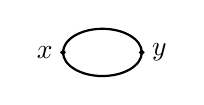
\begin{tikzpicture}[thick,scale=0.5] 
\filldraw (-1,0) circle (1pt) node[left] {$x$};
\filldraw (1,0) circle (1pt) node[right] {$y$};
\draw (0,0) circle (1cm and 0.6cm);
\end{tikzpicture}
\end{figure}
\end{minipage}
\hspace*{-8pt}
$\longrightarrow$
\hspace{5pt}
\begin{minipage}{0.7\linewidth}
\vspace*{-13pt}
\begin{equation*}
\Delta_\fsf^2(x,y) = \frac{1}{8 \pi^2} \bigg( \frac{u^2(x,y)}{\sigma_\fsf^2(x,y)} +  
\mbox{``well defined for $x=y$''}
\bigg)
\end{equation*}
\end{minipage}

\vspace*{20pt}

$\bullet$ regularize only $\sigma_\fsf^{-(2+\alpha)}$ \\

$\bullet$ use $\sigma$ identities : \ $ \Box \sigma = 4 + f \sigma $ \\
 
$\bullet$ $\alpha \mapsto \sigma_\fsf^{-(2+\alpha)}$ (weakly) meromorphic in $\alpha$. \\
\quad $\to$ Laurent series w.r.t $\alpha$ \\
\quad $\to$ subtract the principal part and take the limit $\alpha \to 0$
 
\begin{equation*}
\left(\frac{1}{\sigma_\fsf^2}\right)_\mathsf{reg} \ = \ \lim_{\alpha \to 0} \ \left( 1 - \pp \right) \frac{1}{\sigma_\fsf^{2+\alpha}} 
\end{equation*}
\begin{equation*}
\Longrightarrow \ \left(\Delta_\fsf^{2}\right)_\mathsf{reg} 
\end{equation*}
 
\end{frame}

%----------------------------------------------------------------------------%
\section{ncft}
%----------------------------------------------------------------------------%

{
\setbeamertemplate{footline}{} 
\setbeamertemplate{headline}{}
\setbeamertemplate{background}{\includegraphics[width=\paperwidth,height=\paperheight]{fig_flwr}}
\pgfsetfillopacity{0.8}
\begin{frame}
\bf
\begin{exampleblock}{\vspace*{-3ex}}
\begin{center}
\Large Noncommutative field theory \\ A three dimensional gauge model
\end{center}
\end{exampleblock}
\end{frame}
}

%----------------------------------------------------------------------------%

\begin{frame}
 
\frametitle{The Wick Voros space} 

\vfill

\textbf{An euclidean space}
\vspace*{-10pt}
\begin{equation*}
\mathbb{R}^3_\lambda = \mathbb{C}[x_0,x_1,x_2,x_3] \backslash \mathcal{I}\left[\mathcal{R}_1,\mathcal{R}_1\right]
\end{equation*}

where $\mathbb{C}[x_0,x_1,x_2,x_3]$ is the free algebra generated by $x_{i=1,2,3}$ and $x_0$ \\
and $\mathcal{I}\left[\mathcal{R}_1,\mathcal{R}_1\right]$ is the two sided ideal generated by the relations
\vspace*{-10pt}
\begin{equation*}
\mathcal{R}_1 : [x_i,x_j] = i \lambda \epsilon_{ijk} x_k \ , \quad \mathcal{R}_2 : x_0^2 + \lambda x_0 = \sum_{i=1}^3 x_i^2
\end{equation*}

\vfill

\textbf{Basis}
\vspace*{-10pt}
\begin{equation*}
\phi \in \mathbb{R}^3_\lambda\ , \qquad \phi = \sum_{j\in\frac{\mathbb{N}}{2}} \left( \sum_{m,n=-j}^j \phi^j_{m n} v^j_{m n} \right)
\end{equation*}

with $\phi^j_{m n} \in \mathbb{C}$ and $\{v^j_{m n}\}$ the natural orthogonal basis of $\mathbb{R}^3_\lambda$
 
\vfill

\textbf{Scalar product}  
\vspace*{-10pt}
\begin{equation*}
\Smearip{\Phi,\Psi} = \mathsf{Tr}\left( \Phi^\dagger \Psi \right) = 8 \pi \lambda^3 \sum_{j\in\frac{\mathbb{N}}{2}} \ (j+1) \sum_{m,n=-j}^j \phi^j_{n m} \ \psi^j_{m n}
\end{equation*}

\end{frame}

%----------------------------------------------------------------------------%

%----------------------------------------------------------------------------%

\begin{frame}
 
\frametitle{The Classical actions} 

\vfill

$\to$  we need a notion of ``noncommutative connection'' to define gauge field

\vfill

\textbf{Lie algebra of real inner derivations} of $\mathbb{R}^3_\lambda$
\begin{equation*}
\mathcal{G} = \left\{ D_i \cdot = i \left[\frac{x_i}{\lambda^2} , \cdot \right], \ \forall i =1,2,3 \right\}
\end{equation*}

\vfill

\textbf{connection} on $\mathbb{R}^3_\lambda$ can be defined as linear map $\nabla : \mathcal{G} \times \mathbb{R}^3_\lambda \to \mathbb{R}^3_\lambda$, with
\begin{equation*}
\nabla_{D_i} (a) = D_i(a) + A_i a \ , \quad \mbox{with } \ A_i = \nabla_{D_i}(\mathbb{I}) \ \to \ \mbox{ gauge field !}
\end{equation*}

\vfill

\textbf{gauge transformation}: $A_i^g = g^\dagger A_i g + g^\dagger D_i g$ 
\vspace*{-2pt}
\begin{eqnarray*}
&\mbox{ invariant gauge connection : } \nabla_{D_i}^{inv} (a) = - i a \frac{x_i}{\lambda^2}& \\
&\Phi_i = i( \nabla^{inv}_{D_i} - \nabla_{D_i})  \ \to \ \Phi_i^g = g^\dagger \Phi_i g&
\end{eqnarray*}

\vfill

\textbf{The classical actions}
\vspace*{-6pt}
\begin{equation*}
\Ssf(\Phi) = \frac{1}{g^2} \mathsf{Tr}\left( \alpha \Phi_i\Phi_j\Phi_j\Phi_i + \beta \Phi_i\Phi_j\Phi_i\Phi_j + i \xi \epsilon_{ijk} \Phi_i\Phi_j\Phi_k + (M+\mu x^2) \Phi_i\Phi_i \right) 
\end{equation*}

\vfill
 
\end{frame}


%----------------------------------------------------------------------------%

\begin{frame}

\frametitle{Gauge fixing -- Propagator}

\vfill

$\to$ particular choice of the parameter in the action (ta make life easier \smiley )

\vfill

\textbf{Gauge fixing} (fixe the freedom whci remains) :  BRST \\
we choose $\Phi_3 = x_3$
\vspace*{-6pt}
\begin{eqnarray*}
&\dots \mbox{ (after a bit of computations) } \dots& \\
&\Ssf(\Phi) = \frac{1}{g^2} \mathsf{Tr}\left( \Phi_1 K \Phi_1 + \Phi_2 K \Phi_2 \right) + \frac{4}{g^2} \mathsf{Tr}\left(\left(\Phi_1^2 + \Phi_2^2\right)^2\right) &
\end{eqnarray*}

\vfill

\textbf{Propagator of the full theory}
%
\begin{equation*}
P = \frac{1}{(j+1)\left( M + \mu \lambda^2 j (j+1) + \lambda^{-2} (k^2+l^2) \right)}
\end{equation*}


\textbf{Propagator of the troncated theory} (whitout the field $\Phi_3$)
%
\begin{equation*}
Q = \frac{1}{(j+1)\left( M + \mu \lambda^2 j (j+1) \right)}
\end{equation*}

\vfill 
 
\end{frame}


%---------------------------------------------------------------------------

\begin{frame}

\frametitle{Theory finite at all orders}

\vfill

\textbf{Truncated theory} \\
$\to$ we look if the amplitude of general diagram is always finite
%
\begin{equation*}
\abs{\mathcal{T}^j} \leq K . (j+1)^{vertex} . (2j+1)^{loop} . Q^{intern \ lines} \leq K^\prime \frac{(j+1)^{V-I}.(2j+1)^{\ell}}{(M^\prime+j^2)^I}
\end{equation*}

$\bullet$ \ $j=0$ \ : finite ! \\

$\bullet$ \ $j\to\infty$ \ : finite because we have $3I-V-\ell \geq 0$.

\vfill

\textbf{Full theory} \\
the following estimate holds true
\begin{equation*}
0\leq P \leq Q 
\end{equation*}
therefore
\begin{equation*}
\abs{\mathcal{F}^j} \leq \sum_{k_1,\dots,k_n=-j}^{j} \ \ \prod_{intern \ lines} \abs{P^j} \ \abs{f^j(\delta)} \leq \sum_{k_1,\dots,k_n=-j}^{j} \ \ \prod_{intern \ lines} \abs{Q^j} \ \abs{f^j(\delta)} \leq \infty
\end{equation*}

\vfill

\end{frame}

%----------------------------------------------------------------------------%
\section{Conclu.}
%----------------------------------------------------------------------------%

{%
\setbeamertemplate{footline}{} 
\setbeamertemplate{headline}{}
\setbeamertemplate{background}{\includegraphics[width=\paperwidth,height=\paperheight]{fig_conclu}}
\pgfsetfillopacity{0.88}
\begin{frame}
\vfill
\begin{flushright}
\textcolor{white!80!blue}{\bf \LARGE Grazie.}
\end{flushright}
\end{frame}
}%

%----------------------------------------------------------------------------%
\appendix
\backupbegin
%----------------------------------------------------------------------------%

%\begin{frame}[label=blablabla]

%\frametitle{blablabla}
 
%\hfill \hyperlink{blablabla}{\beamerreturnbutton{back}}

%\end{frame}

%----------------------------------------------------------------------------%
\backupend
%----------------------------------------------------------------------------%

%============================================================================%
\end{document} 
%============================================================================%